\documentclass[]{book}

\usepackage{import}
\usepackage{preamble}

\begin{document}

\noindent BECA / Huson / 11.1 IB Math SL \hspace{2in} Name:\\*
6 October 2017
\begin{center}
{\Large Functions and Quadratics Review}\\
\textit{Materials covered in the next test. Due Tuesday}
\end{center}

%\vspace{0.2 cm}


\section*{Solve for the roots or zeros of a quadratic function, $f(x)=0$}

\subsection*{Factoring}

Solve for the roots of the function by factoring.

\begin{enumerate}

\item   $f(x)=x^2-4x$
\item   $f(x)=-2x^2+10x$
\item   $f(x)=x^2-9x+18$
\item   $f(x)=x^2-8x-20$
\item   $f(x)=2x^2-7x-30$
\item   $f(x)=\frac{7}{10}(x^2+12x-45)$

\subsection*{Completing the square}

Rewrite the function in vertex form, $f(x)=a(x-h)^2+k$. Include the step showing the $(-\frac{b}{2a})^2$ term. State the vertex as an ordered pair and the equation for the axis of symmetry.
\item   $f(x)=x^2+10x+14$
\item   $f(x)=x^2+8x+11$
\item   $f(x)=-(x^2+2x-3)$

\subsection*{Using the quadratic formula}

Solve using the quadratic formula.
\item   $x^2+5x+5=0$
\item   $x^2+5x = 2$
\item   $x^2+7x -7 = 2x^2$

\newpage
\subsection*{Sketching a quadratic function}
Expand the function from vertex form to standard form, $ax^2+bx+c \text{ where } a, b, c \;  \epsilon \; \mathbb{R}$. Then factor the result and state the roots. Sketch the function, labeling the intercepts with values and the vertex as an ordered pair. Show the axis of symmetry as a dotted line and label it with its equation.
\item   $f(x)=-(x+1)^2+4$
\begin{figure}[!ht]
    \flushright
    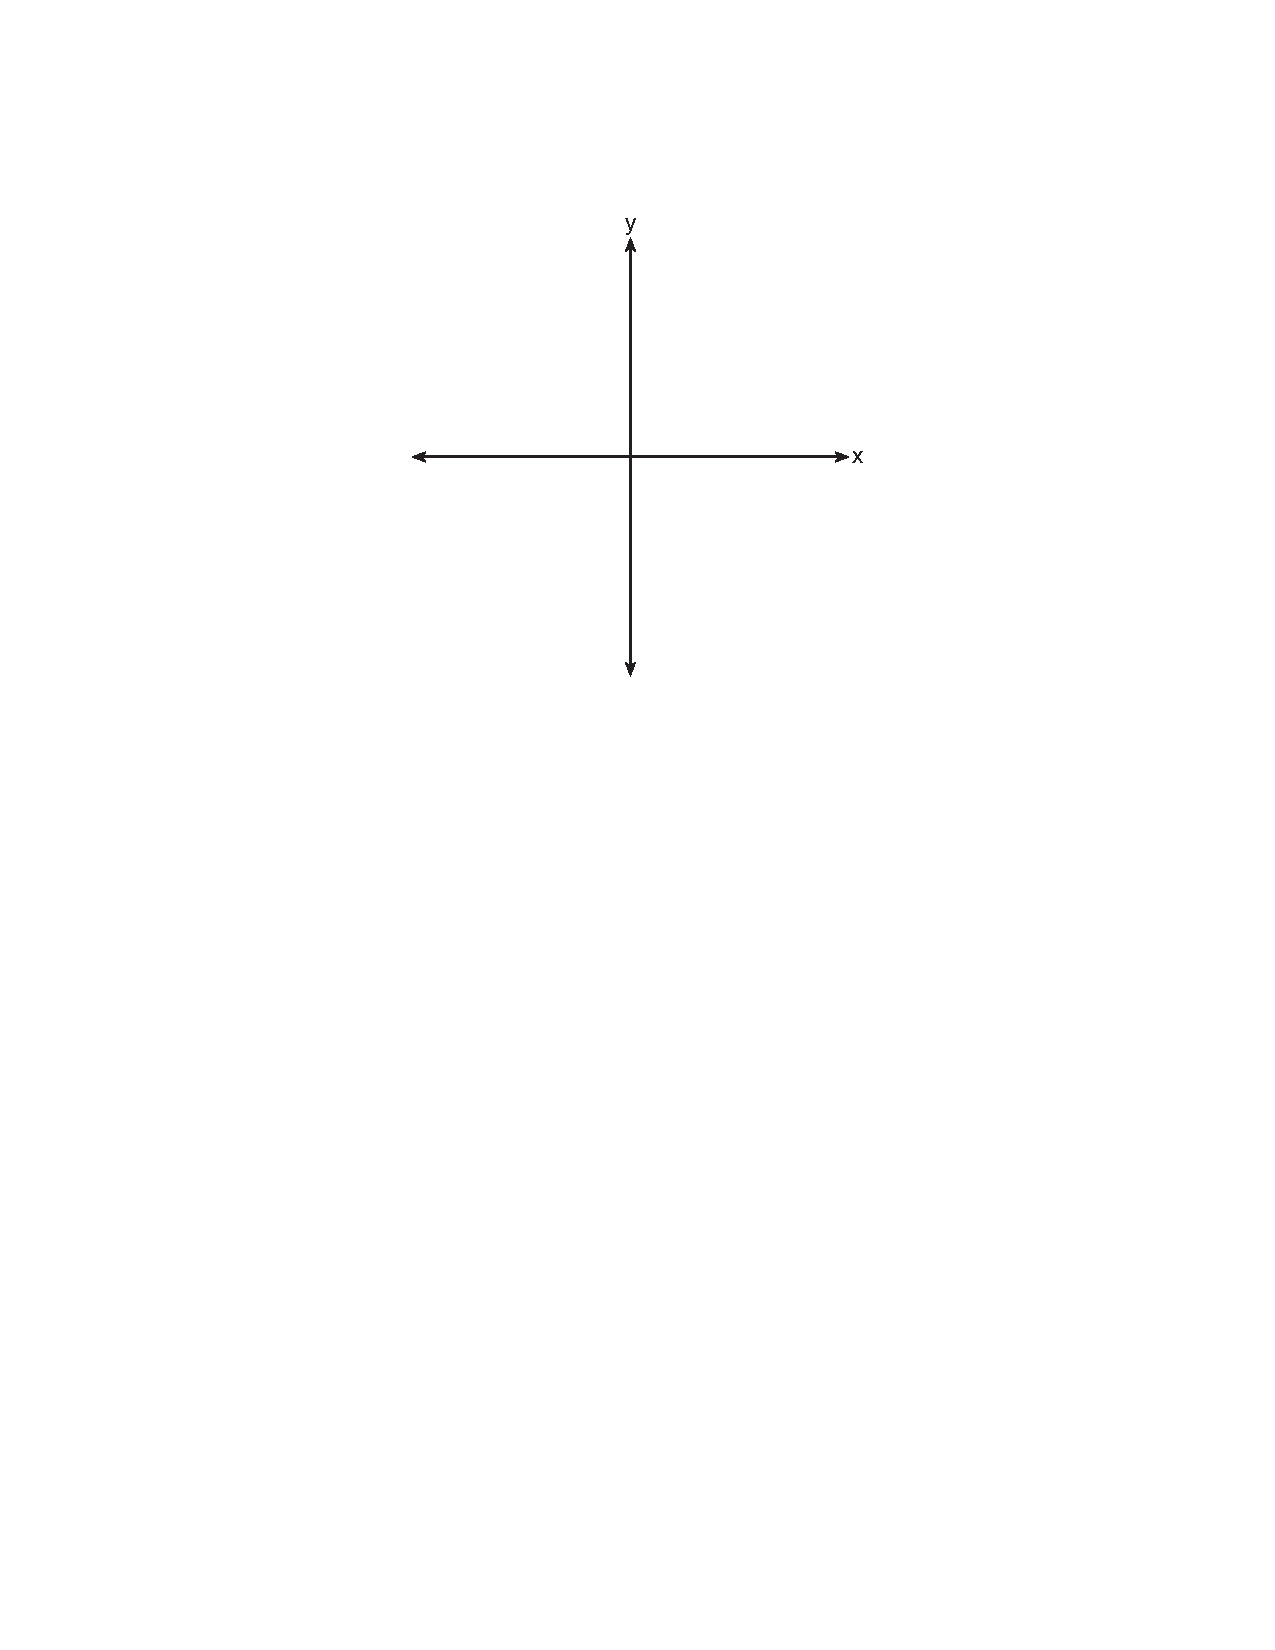
\includegraphics[width=0.65\textwidth]{simple-axes.pdf}
\end{figure}

\item   $f(x)=\frac{1}{2}(x-4)^2-8$\\*
(sketch your own axes for this plot)

\newpage
\subsection*{Graphing quadratics}
\item Graph the function $f(x)=-2x^2-4x+3$. You may use a graphing calculator rather than factoring the function and completing the square.\\*[5pt]
Label the scales with at least a few values. Mark the vertex as an ordered pair and label each intercept with its value. Plot the axis of symmetry as a dotted line and label it with its equation.\\*[20pt]

\begin{figure}[!ht]
    \centering
    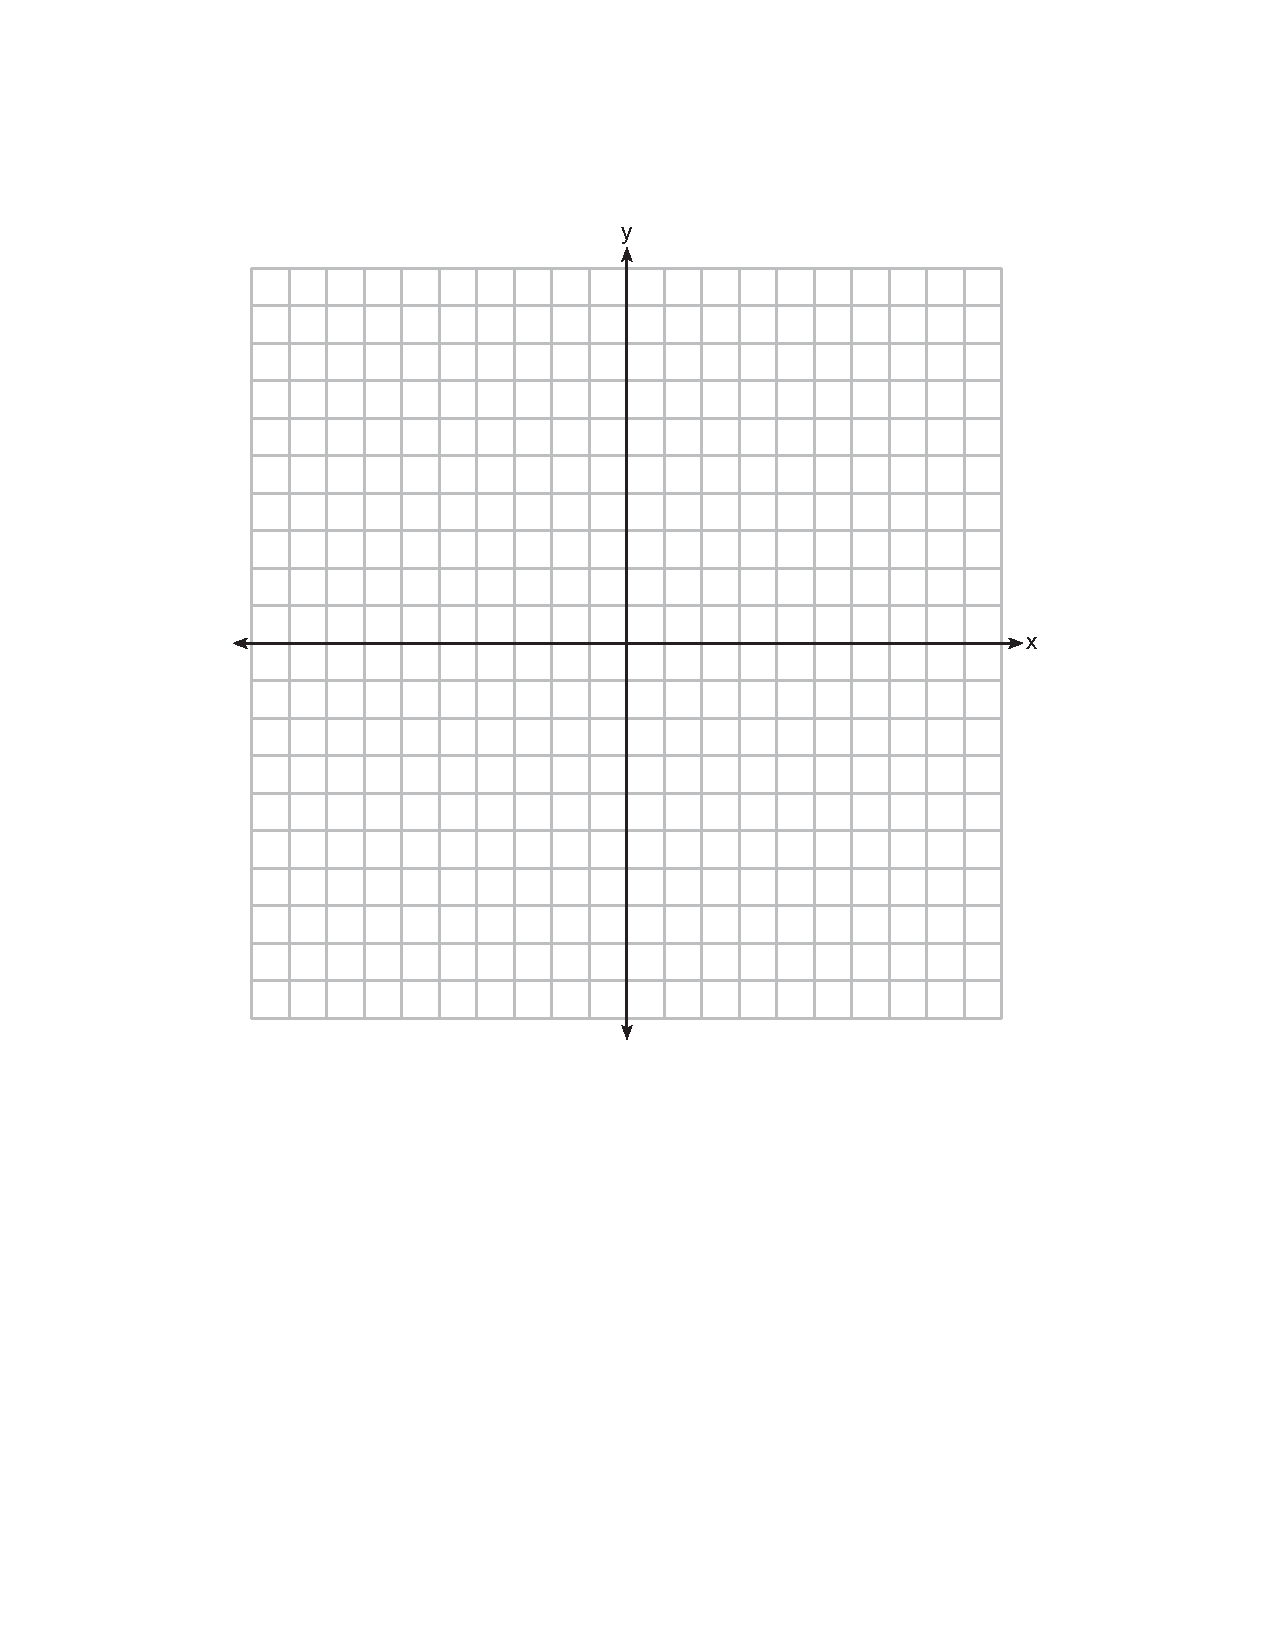
\includegraphics[width=0.75\textwidth]{regents-grid.pdf}
\end{figure}

\newpage
\subsection*{Model situations with quadratic functions}

The path of a diver is given by 
\[y=-\frac{4}{9}x^2+\frac{24}{9}x+12\]
where $y$ is the height (in feet) and $x$ is the horizontal distance from the end of the diving board (in feet).\\*[5pt]
\begin{enumerate}
    \item Use a graphing calculator to view the graph and a table of values. On the grid below, graph the function over the domain $x \geq 0$ and where $y \geq 0$. Use a horizontal scale of 1 square equals six inches and vertical scale of 1 square equals one foot. Label the intercepts and vertex.
    \item What is the maximum height of the diver?\\*[30pt]
    \item What is the diver's horizontal distance to the point she enters the water?\\*[30pt]
\end{enumerate}

\begin{figure}[!ht]
    \flushright
    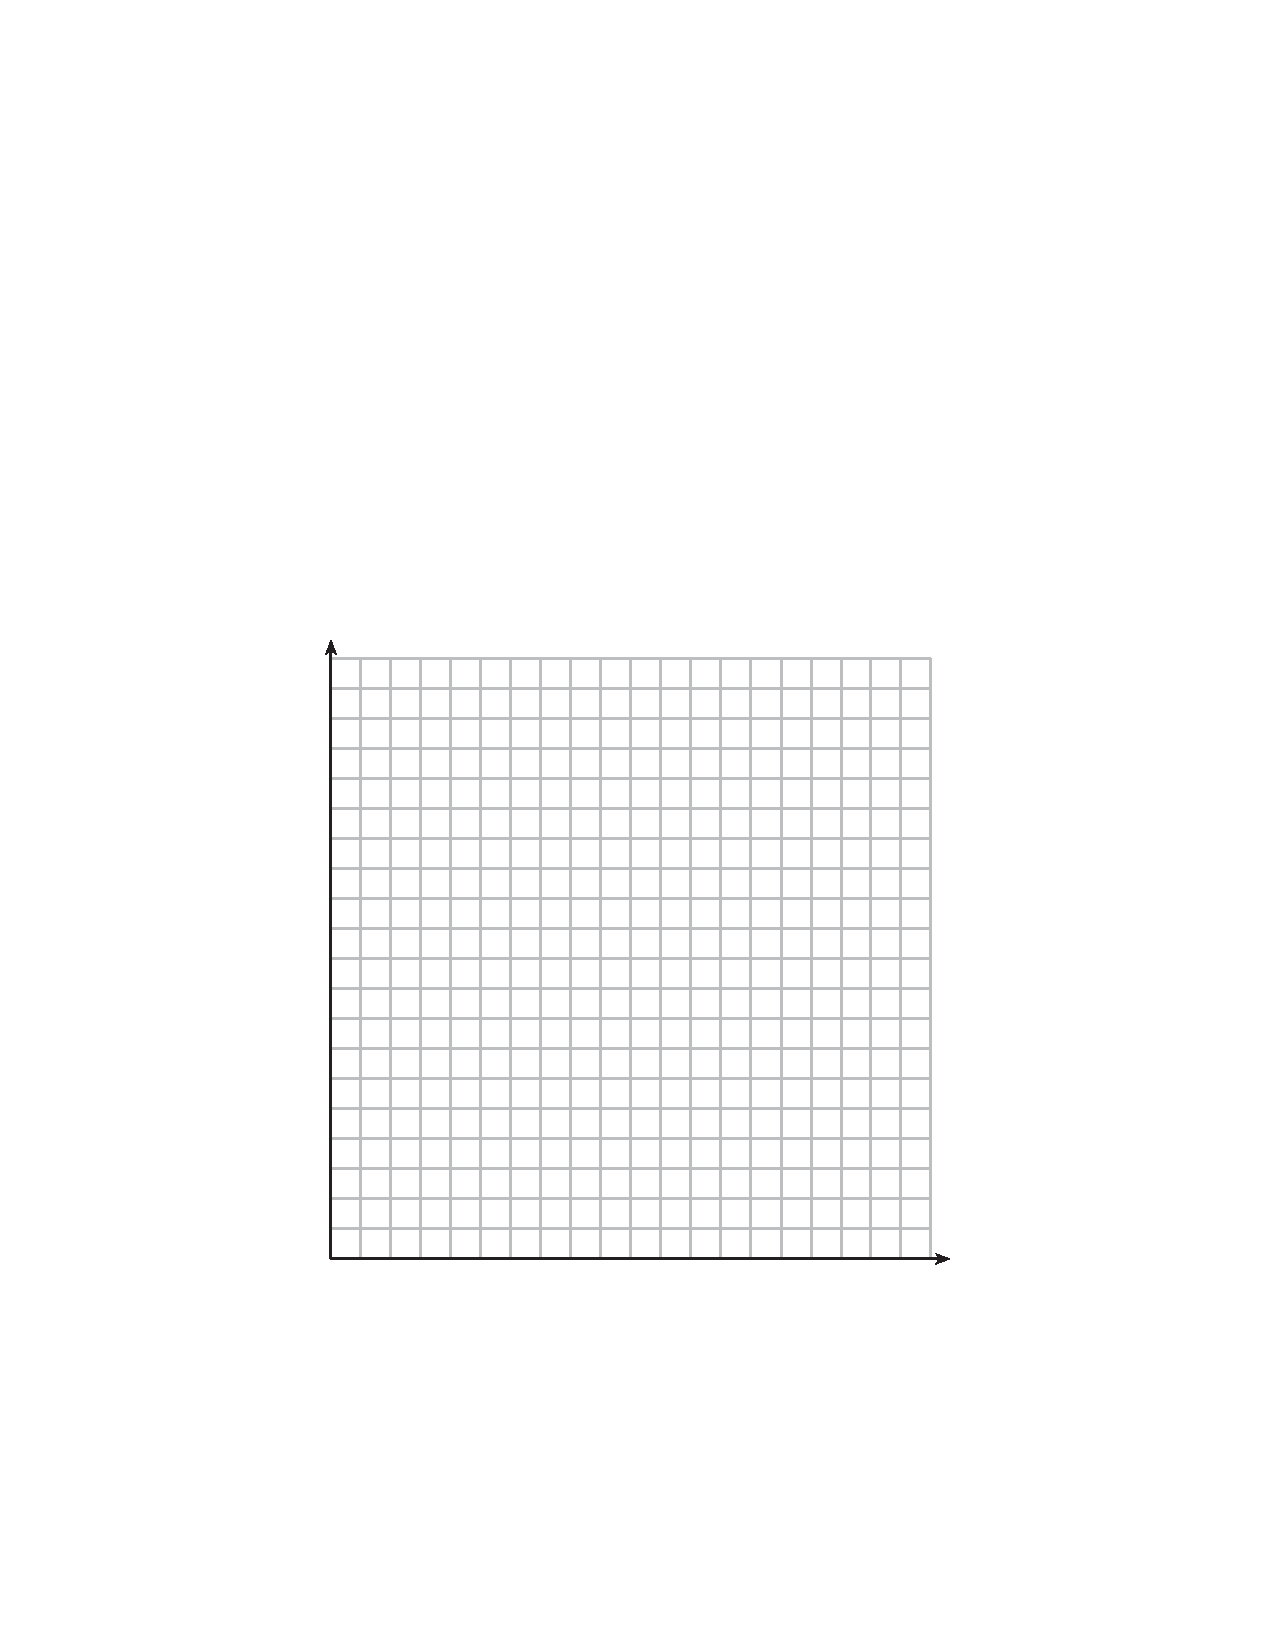
\includegraphics[width=0.65\textwidth]{1stQ-grid.pdf}
\end{figure}

\newpage

\subsection*{The inverse of a function}
Derive the inverse of each function. Simplify the expression.
\item   $f(x)=\frac{1}{3}x-12$
\item   $f(x)=\frac{2}{3}(x-1)^2-5$
\item   $f(x)=\sqrt{x-1}-\frac{3}{2}$

\subsection*{Function substitution}
\item Given $f(x)=x^2+x+1$. Simplify $f(-2x)$?
\item Given $f(x)=x(2x-1)$. Simplify $f(x-11)$?
\item Given $f(x)=1-(2x^2+x)$. Simplify $f(\frac{3}{4}x-3)$?

\subsection*{Function composition}
In each exercise, perform the composition $f \circ g$ and simplify.
\item Given $f(x)=\frac{1}{2}x^2+1$ and $g(x)=\sqrt{x}$
\item Given $\displaystyle f(x)=\frac{1}{x-4}$ and $\displaystyle g(x)=\frac{1}{x}+4$
\item Given $\displaystyle f(x)=\frac{1-x}{x^2}+1$ and $g(x)=3x-3$

\subsection*{Domain and range of a function}
State the domain and range of each function 
\item $f(x)=(x-3)^2-14$
\item $g(x)=\sqrt{x+2}+3$
\item The function graphed below.\\*[5pt]

\begin{figure}[!ht]
    \centering
    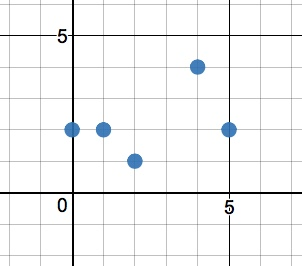
\includegraphics[width=0.35\textwidth]{discrete-domain-graph.jpeg}
\end{figure}


\end{enumerate}
\end{document}